\section{Conclusioni}
        Possiamo concludere che, a meno di un errore del 2-3\%, la misura della carica di un elettrone sia eseguibile tramite la metodologia da noi utilizzata.\\
        Dobbiamo considerare che la misura universalmente oggi accettata è frutto di molte più misurazioni di quelle prese dal nostro gruppo, con strumenti più raffinati e precisi.\\
        Tramite un'analisi statistica più consistente ed un più accurato rigetto dei dati abbiamo ottenuto che la carica elettrica dell'elettrone ha un valore:
        $$q_{e^-} = \left(-1.607\pm0.012\right)\cdot10^{-19}~\mathrm{C}$$
        Calcolando la discrepanza standardizzata del dato sperimentale rispetto al valore atteso, si ottiene che la carica dell'elettrone sperimentalmente ha un livello di confidenza pari a $0.43\sigma$ e una compatibilità del $92.80\%$ con la misura universalmente accettata.\\
        Dobbiamo anche ammettere di aver ottenuto una così grande compatibilità a causa della qualità delle nostre misurazioni, che ci hanno portato a ottenere un errore del $7.4\%$ sulla misura finale.\\
        Consideriamo tale errore accettabile al fine di un'esperienza di laboratorio didattica, ma non si tratta sicuramente di una misurazione estremamente accurata dal punto di vista sperimentale.\\
        Se dovessimo ripetere l'esperimento, la nostra idea sarebbe quella di scegliere con maggiore attenzione le gocce da analizzare. Cercheremmo di evitare di considerare gocce che si muovo troppo velocemente quando è presente il campo elettrico, in modo che l'errore legato al tempo di reazione umano sia il più piccolo possibile rispetto alla misura di tempo.\\
        Questo permetterebbe di ridurre il numero di cariche scartate e quindi di ridurre la deviazione standard della media, avendo un numero maggiore di dati.\\
        La scelta di prendere la temperatura per ogni goccia può essere utile se le misure vengono fatte in istanti di tempo distanti; nel nostro caso, avendo effettuato tutte le misure di seguito, non era così necessario, ma sarebbe bastato prenderla ad intervalli di tempo di $15-20min$.\\
        \subsection{Grafico comparativo, carica effettiva/carica misurata}
\begin{figure}[H]
    \centering
    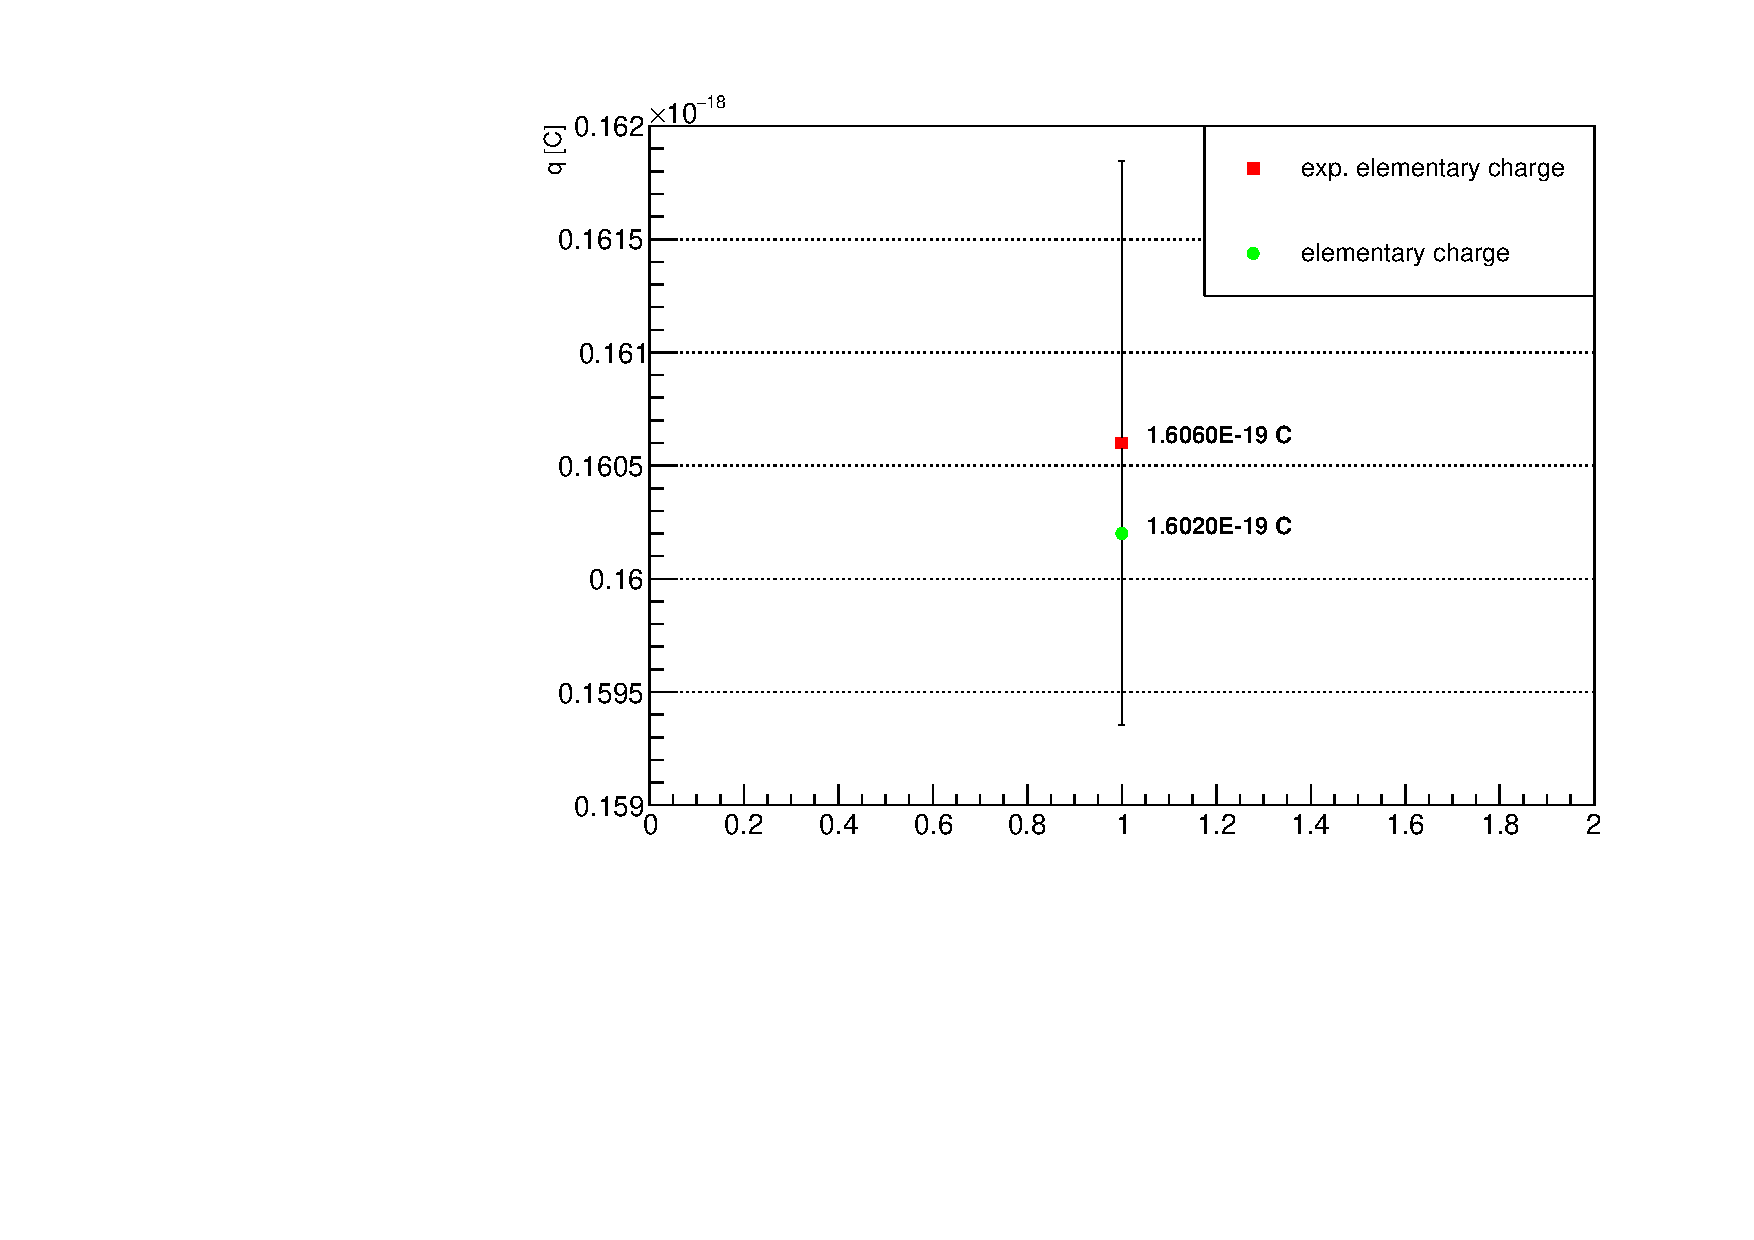
\includegraphics[width=\textwidth,height=\textheight,keepaspectratio]{graph2.pdf}
    \caption{Grafico carica misurata rispotto a carica effettiva}
\end{figure}